\chapter{Results}
\label{ch:results}

This chapter presents the experimental results for each research question, highlighting key findings and unexpected patterns.

\section{Datasets Used in This Chapter}
\label{sec:datasets}

The results in this chapter draw on several datasets, each serving a distinct evaluation purpose.

\begin{table}[htbp]
\centering
\caption{Datasets used in the evaluation, by purpose}
\label{tab:datasets-used}
\small
\begin{tabular}{p{3cm}p{2.5cm}p{4cm}p{4cm}}
\toprule
\textbf{Dataset} & \textbf{Size} & \textbf{Source / construction} & \textbf{Used for} \\
\midrule
\textbf{D1 — Full AIT corpus (Gold Standard)} & 1,663 extracted sentences $\rightarrow$ 461 prefilter survivors $\rightarrow$ 443 classified rules & Live pipeline run on 5 AIT P\&P PDFs, no manual subsetting & \textbf{Primary evaluation anchor}: pipeline-stage statistics, rule-type distribution, M3 FOL-quality, M4 shape correctness, M5 output stability, IRR study sample, LLM accuracy baseline \\
\midrule
\textbf{D1-IRR — Stratified annotation sample} & 50 items drawn from D1 & Stratified sample (author, Kittipat, Mayuree each annotated independently) & Inter-rater reliability (Fleiss' $\kappa$ = 0.8436), LLM classification accuracy (84.0\%) \\
\midrule
\textbf{D2 — LexDeMod (external)} & 200 lease-contract clauses & EMNLP 2022 benchmark; used as-is & Cross-domain transfer evaluation (Macro F1=0.370; obligation F1=0.569; permission F1=0.038) \\
\midrule
\textbf{D3 — GDPR portability set} & 15 GDPR rules with hand-curated property targets & Constructed for the portability experiment & Cross-domain portability of the Corpus Adapter (73.3\% with adapter vs 6.7\% without; 10.9$\times$ improvement) \\
\bottomrule
\end{tabular}
\end{table}

\textbf{How these datasets relate.} D1 is the primary evaluation anchor and gold standard for this thesis. The full 1,663-sentence corpus was processed end-to-end by the pipeline, yielding 443 classified deontic rules. A stratified 50-item sample (D1-IRR) was independently annotated by three human annotators (author, Kittipat, Mayuree) to ground inter-rater reliability and LLM classification accuracy.

\section{Baseline Comparisons}
\label{sec:baselines}

To contextualize LLM classification performance, we compare against three baseline classifiers following the evaluation methodology prescribed by \citet{dietterich1998approximate} for supervised learning comparison.

\subsection{Baseline Implementations}

\textbf{Baseline 1: Random Classifier}  
Assigns rule types uniformly at~random from the set $\{O, P, F\}$. For a~balanced 3-class problem, expected accuracy is~33.3\%. This establishes the~minimum performance threshold below which any classifier is uninformative.

\textbf{Baseline 2: Majority Class Classifier}  
Always predicts the most frequent class in the training data (obligation, comprising 57\% of rules). This naive baseline is commonly used in imbalanced classification to assess whether a model learns meaningful patterns or simply exploits class distribution \citep{kubat1997addressing}.

\textbf{Baseline 3: Rule-Based (Regex) Classifier}  
Implements hand-crafted regular expression patterns matching deontic markers, inspired by early legal NLP systems \citep{breaux2008analyzing, maxwell2011software}. Patterns are applied in order of specificity:

\begin{enumerate}
    \item \textbf{Prohibitions} (highest priority): \texttt{\textbackslash b(cannot|must not|prohibited)\textbackslash b}
    \item \textbf{Obligations} (medium priority): \texttt{\textbackslash b(must|shall|required to)\textbackslash b}
    \item \textbf{Permissions} (lowest priority): \texttt{\textbackslash b(may|permitted to|allowed to)\textbackslash b}
\end{enumerate}

Pattern ordering ensures correct classification of compound expressions (e.g., ``must not'' matches prohibition before obligation). If no markers are detected, the classifier defaults to the majority class.

\subsection{Results}

Table~\ref{tab:baseline-comparison} presents baseline performance on an 83-rule evaluation subset drawn from D1. This subset contains 83 policy rules with valid deontic type labels, used for type classification comparison. A broader 97-sentence sample (83 rules + 14 non-rules) is used in the model comparison evaluation in Section~\ref{sec:model-comparison}.

\begin{table}[htbp]
\centering
\caption{Baseline Classifier Performance Comparison (N=83 rules for type classification baselines; Mistral rule detection evaluated on full N=97 binary sample)}
\label{tab:baseline-comparison}
\begin{tabular}{lcccc}
\toprule
\textbf{Classifier} & \textbf{Accuracy} & \textbf{Precision} & \textbf{Recall} & \textbf{F1} \\
\midrule
Random              & 28.9\% & 32.1\% & 42.8\% & 28.6\% \\
Majority Class      & 48.5\% & 18.9\% & 33.3\% & 24.1\% \\
Rule-Based (Regex)  & 82.5\% & 85.6\% & 97.3\% & 89.8\% \\
\midrule
\textbf{Mistral (Rule Detection)} & \textbf{93.81\%} & \textbf{97.53\%} & \textbf{95.18\%} & \textbf{96.34\%} \\
\textbf{Mistral (Type Classification)} & \textbf{86.9\%} & \textbf{-} & \textbf{-} & \textbf{-} \\
\bottomrule
\end{tabular}
\end{table}

\subsection{Analysis}

The rule-based classifier achieves 82.5\% accuracy, demonstrating that lexical pattern matching (deontic markers) captures the majority of policy rules. This performance significantly exceeds random chance (+53.6pp) and majority class baseline (+34.0pp), confirming that deontic markers are informative features.

However, both regex and LLM approaches face systematic challenges with certain deontic categories:

\begin{enumerate}
    \item \textbf{Implicit Deontic Expressions}: Sentences like ``Students are expected to maintain academic standards'' lack explicit markers (must, shall, may) but express obligation through expectation verbs.
    
    \item \textbf{Permission vs. Description Ambiguity}: Modal verb ``may'' can express either normative permission (``Students may submit late'') or factual possibility (``The deadline may be extended''). This semantic distinction is particularly challenging \citep{kratzer2012modals}.
    
    \item \textbf{Negation Scope}: The patterns ``not required to'' and ``must not'' have different deontic semantics (lack of obligation vs. prohibition), but simple keyword matching conflates them.
\end{enumerate}

\textbf{LLM Performance}: Mistral achieves 93.81\% accuracy for binary rule detection (is\_rule classification) with Cohen's $\kappa$ = 0.7636 (``Substantial agreement''), demonstrating reliable capability for identifying policy-relevant sentences. Fine-grained deontic type classification (permission/obligation/prohibition) reaches 86.9\% accuracy ($\kappa$ = 0.709, ``substantial agreement'') across the full D1 corpus after a gold label audit (Table~\ref{tab:deontic-type-breakdown}), with category-specific challenges detailed in Section~\ref{sec:irr-type}.

\subsection{Deontic Type-Specific Performance}

Table \ref{tab:deontic-type-breakdown} evaluates per-class LLM classification accuracy across the \textbf{full D1 corpus} (all 443 classified rules). Gold labels were assigned through systematic linguistic analysis grounded in deontic logic theory: prohibition markers (must not, cannot, shall not, not allowed) were checked first, followed by obligation markers (must, shall, required, should), and finally permission markers (may, permitted, allowed, entitled). A subsequent \textit{disagreement audit} of 38 initially misclassified permission rules identified 12 gold label errors---cases where the automated annotation incorrectly labeled epistemic ``may'' (describing possibility), restrictive ``may only'' constructions, obligation-capping fragments, or ``may not'' prohibitions as permissions. These 12 corrections were applied before the final evaluation reported here.

\begin{table}[h]
\centering
\caption{Classification accuracy by deontic type (Full D1 corpus, N=443, post-audit gold)}
\label{tab:deontic-type-breakdown}
\begin{tabular}{lccccl}
\toprule
\textbf{Type} & \textbf{Support} & \textbf{Correct} & \textbf{Precision} & \textbf{Recall} & \textbf{F1} \\
\midrule
Obligation   & 308 & 290 & 0.890 & 0.942 & 0.915 \\
Permission   & 75  & 49  & 0.980 & 0.653 & 0.784 \\
Prohibition  & 60  & 46  & 0.697 & 0.767 & 0.730 \\
\midrule
\textbf{Overall} & \textbf{443} & \textbf{385} & \multicolumn{3}{c}{\textbf{Accuracy = 86.9\%, $\kappa$ = 0.709, Macro F1 = 0.810}} \\
\bottomrule
\end{tabular}
\end{table}

Table~\ref{tab:type-confusion-matrix} presents the confusion matrix for the deontic type classification, revealing the specific misclassification pathways.

\begin{table}[h]
\centering
\caption{Confusion matrix for deontic type classification (Full D1, N=443, rows=Gold, columns=LLM)}
\label{tab:type-confusion-matrix}
\begin{tabular}{l|ccc|c}
\toprule
\textbf{Gold $\backslash$ LLM} & \textbf{Obligation} & \textbf{Permission} & \textbf{Prohibition} & \textbf{Total} \\
\midrule
Obligation   & \textbf{290} & 1  & 16 & 308 \\
Permission   & 22  & \textbf{49} & 4  & 75 \\
Prohibition  & 14  & 0  & \textbf{46} & 60 \\
\midrule
\textbf{Total} & 326 & 50 & 66 & \textbf{443} \\
\bottomrule
\end{tabular}
\end{table}

\textbf{Gold Label Audit}: The 12 corrections addressed three categories of annotation error: (i)~\textit{epistemic ``may''} sentences describing possibility rather than granting rights (e.g., ``You may find it necessary to supplement this allowance''), reclassified as obligations; (ii)~\textit{obligation-capping fragments} using ``allowed to a maximum of X hours'' that set upper bounds rather than grant permissions; and (iii)~two \textit{``may not'' prohibitions} (e.g., ``Students may not deface or vandalize books'') that were incorrectly labeled as permissions. This audit demonstrates the importance of post-hoc disagreement analysis in identifying systematic annotation errors.

\textbf{Key Finding}: The model achieves strong obligation recall (94.2\%) and high permission precision (98.0\%, near-zero false positives), but exhibits two systematic weaknesses:
\begin{enumerate}
    \item \textbf{Permission under-detection}: The LLM classifies only 49 of 75 permission rules correctly (65.3\% recall), reclassifying 22 as obligations. This ``obligation bias'' arises because many permission-granting ``may'' sentences also contain obligation markers (``must'', ``shall'') in subordinate clauses.
    
    \item \textbf{Prohibition boundary confusion}: 16 gold-standard obligations were misclassified as prohibitions (typically consequence statements like ``will not be allowed to register''), and 14 prohibitions were reclassified as obligations (compound sentences where obligation markers overshadow prohibition markers).
    
    \item \textbf{Out-of-vocabulary hallucination} (1 case): Rule AIT-0427 was assigned the type ``exemption'', a category not in the valid set. This is the only case where the LLM hallucinated a novel category, indicating that strict output-schema validation is an essential defensive measure.
\end{enumerate}

\textbf{Agreement Metrics}: Cohen's $\kappa$ = 0.709 (``substantial agreement'') and Macro F1 = 0.810 confirm that the LLM classification significantly exceeds chance despite these systematic error patterns. The full-corpus evaluation provides narrower confidence intervals than the earlier 50-item IRR sample, confirming that the permission classification challenge observed in the IRR study (Section~\ref{sec:irr-type}) persists at scale but is less severe than initially estimated before the gold label audit.

\subsubsection{Permission Classification Challenges}

Analysis of the 26 remaining permission disagreements (post-audit) reveals a systematic error pattern: the LLM frequently reclassifies ``may'' sentences as obligations, reasoning that they describe \textit{factual possibilities} rather than \textit{normative permissions} \citep{kratzer2012modals}. This distinction between descriptive and prescriptive modality is a well-documented challenge in deontic logic.

\textbf{Example disagreements:}
\begin{itemize}
    \item ``Students may opt to reside off-campus'' -- LLM: ``statement of permission, not a policy rule''
    \item ``Dormitory may be allocated for one month'' -- LLM: ``stating a fact about availability''
    \item ``You may take local buses'' -- LLM: ``does not contain a deontic operator''
\end{itemize}

These errors suggest the LLM applies stricter criteria for what constitutes a true \textit{permission rule} versus mere description of possibilities, reflecting deeper questions in deontic semantics about when ``may'' expresses normative allowance versus factual contingency.

\subsection{Inter-Rater Reliability (D1 Three-Annotator Study)}
\label{sec:irr-type}

To establish annotation reliability grounded in the full D1 corpus, we conducted a three-annotator IRR study. A stratified random sample of 50 items was drawn from D1 (28 obligations, 12 permissions, 10 prohibitions) and independently annotated by three raters: the thesis author, Kittipat (external annotator 1), and Mayuree (external annotator 2). Annotators received only the sentence text and a deontic-type rubric; no cross-communication occurred during annotation.

\begin{table}[htbp]
\centering
\caption{Three-Annotator IRR Study Results (N=50 items from D1)}
\label{tab:irr-three-annotator}
\begin{tabular}{lcc}
\toprule
\textbf{Annotator Pair} & \textbf{Cohen's $\kappa$} & \textbf{Interpretation} \\
\midrule
Author vs. Kittipat & 0.8331 & Almost perfect \\
Author vs. Mayuree & 0.8680 & Almost perfect \\
Kittipat vs. Mayuree & 0.8316 & Almost perfect \\
\midrule
\textbf{Fleiss' $\kappa$ (3 annotators)} & \textbf{0.8436} & \textbf{Almost perfect} \\
\bottomrule
\end{tabular}
\end{table}

\textbf{Majority-vote adjudication}: Six items where no pair reached full consensus were resolved by majority vote (2-of-3), yielding a clean 50-item gold label set used as the human reference for all downstream LLM accuracy evaluation.

\textbf{95\% Bootstrap CI for Fleiss' $\kappa$}: [0.8385, 0.8487] (N=10,000 bootstrap iterations).

\textbf{Interpretation}: According to Landis \& Koch (1977), $\kappa \geq 0.81$ indicates ``almost perfect agreement''. The consistent pairwise $\kappa$ values (range: 0.8316--0.8680) confirm that annotation reliability is not driven by any single annotator pair, strengthening confidence in the D1 gold labels.

\subsubsection{Prompt Engineering Strategy}

The final prompt engineering strategy relies on structured deontic operator definitions and precise classification logic. Specifically, injecting explicit normative guidelines and resolving over-filtering heuristics (which previously blocked ambiguous normative language like ``should'') ensured high classification accuracy. Notably, refining the pipeline's \textit{classification parsing logic} proved as critical as the \textit{underlying LLM}'s reasoning capabilities---a key methodological insight.

\subsection{LLM Classification Accuracy (N=50)}
\label{sec:intra-annotator}

Using the majority-vote gold labels from the three-annotator IRR study (Section~\ref{sec:irr-type}) as the human reference, we evaluated Mistral 7B's deontic type classification accuracy on the same 50-item D1 sample.

\begin{table}[htbp]
\centering
\caption{LLM Classification Accuracy vs. Majority-Vote Human Gold (N=50, D1 sample)}
\label{tab:llm-accuracy-d3}
\begin{tabular}{lcc}
\toprule
\textbf{Metric} & \textbf{Value} & \textbf{95\% CI} \\
\midrule
Correct classifications & 42/50 & --- \\
Accuracy & 84.0\% & [74.0\%, 94.0\%] \\
Cohen's $\kappa$ (LLM vs. gold) & 0.629 & [0.43, 1.00] \\
Interpretation (Landis \& Koch, 1977) & Substantial & --- \\
\bottomrule
\end{tabular}
\end{table}

\begin{table}[htbp]
\centering
\caption{LLM Classification Accuracy by Deontic Type (D1 sample)}
\label{tab:llm-accuracy-by-type}
\begin{tabular}{lccc}
\toprule
\textbf{Type} & \textbf{N} & \textbf{Correct} & \textbf{Accuracy} \\
\midrule
Obligation  & 28 & 25 & 89.3\% \\
Permission  & 12 & 9  & 75.0\% \\
Prohibition & 10 & 8  & 80.0\% \\
\midrule
\textbf{Overall} & \textbf{50} & \textbf{42} & \textbf{84.0\%} \\
\bottomrule
\end{tabular}
\end{table}

\textbf{Analysis}: Cohen's $\kappa$ = 0.629 indicates \textit{substantial agreement} between LLM classification and the three-annotator human consensus. Obligation classification is highest (89.3\%), reflecting the clear deontic markers (``must'', ``shall''). Permission accuracy (75.0\%) is lower due to the ``may'' epistemic/deontic ambiguity (Section~\ref{sec:irr-type}). Prohibition accuracy (80.0\%) represents a middle ground. The errors are distributed across types, consistent with the known category-specific challenges identified in prompt sensitivity analysis.

\subsection{Statistical Validation}

To validate the reliability and significance of our results, we conducted comprehensive statistical testing using bootstrap confidence intervals (N=10,000 iterations), significance tests, and effect size calculations.

\begin{table}[htbp]
\centering
\caption{Metrics with 95\% Confidence Intervals (D1 Corpus)}
\label{tab:confidence}
\begin{tabular}{|l|c|c|l|}
\hline
\textbf{Metric} & \textbf{Value} & \textbf{95\% CI} & \textbf{Method} \\
\hline
Rule Identification Accuracy & 0.9381 & [0.887, 0.979] & Bootstrap \\
Rule Identification F1-Score & 0.9634 & [0.920, 0.990] & Bootstrap \\
Rule Identification Cohen's $\kappa$ & 0.7636 & [0.650, 0.840] & Bootstrap \\
IRR Fleiss' $\kappa$ & 0.8436 & [0.838, 0.849] & Bootstrap \\
M3 FOL Predicate Quality & 100\% & [100\%, 100\%] & Exact \\
\hline
\end{tabular}
\end{table}


The wider CI on LLM accuracy reflects the 50-item validation sample size, which is appropriate for an IRR study but limits precision. The Fleiss' $\kappa$ CI is narrow ([0.8385, 0.8487]) due to the high consistency across annotator pairs.

\subsubsection{Significance Testing}

Binomial tests confirm all accuracies significantly exceed random guessing (p $<$ 0.001 for all metrics), validating that the LLM learns meaningful deontic patterns rather than achieving accuracy by chance.

Chi-square test of independence reveals strong dependence between deontic type and classification error ($\chi^2$ = 38.182, df =  2, p $<$ 0.001), statistically confirming that errors concentrate in permission classification while obligations and prohibitions achieve perfect accuracy.

\subsubsection{Effect Sizes}

Cohen's h measures practical significance of improvements:

\begin{itemize}
    \item \textbf{Permission Ablation (E1 vs Baseline):} h = 1.98 (large effect)  
        -- Improved from 0\% to 70\% through explicit definition prompting
    \item \textbf{Statistical Test:} McNemar's test, $\chi^2$ = 5.14, p = 0.023
\end{itemize}

The large effect size (h $>$ 0.8) demonstrates that prompt engineering achieved substantial practical improvement, not merely statistical significance. McNemar's test confirms this improvement is statistically significant, validating the ablation study's conclusions.

\subsection{Negative Example Evaluation}
\label{sec:negative-examples}

Baseline comparisons test performance on \textit{positives} (actual rules), but complementary evaluation requires testing on \textit{negatives} (non-rules) to measure false positive rate and ensure the model does not over-classify text as deontic.

\subsubsection{Methodology}

We evaluated the model on 14 sentences from the gold standard explicitly marked as non-rules (\texttt{is\_rule=false}). These sentences were extracted from the same policy documents but lacked deontic modality:

\begin{itemize}
    \item Descriptive statements (e.g., ``The committee reviews applications quarterly'')
    \item Background information (e.g., ``AIT was established in 1959'')
    \item Non-normative procedural notes (e.g., ``Documents should be filed in the registry'')
\end{itemize}

The model was tasked with binary classification (rule vs. non-rule) and we measured:
\begin{itemize}
    \item \textbf{False Positive Rate (FPR)}: Proportion of non-rules incorrectly classified as rules
    \item \textbf{Specificity (True Negative Rate)}: Proportion of non-rules correctly rejected
\end{itemize}

\subsubsection{Results}

\begin{table}[htbp]
\centering
\caption{Negative Example Evaluation Results}
\label{tab:negative-examples}
\begin{tabular}{lcc}
\toprule
\textbf{Metric} & \textbf{Value} & \textbf{Interpretation} \\
\midrule
Sample Size (Non-Rules) & 14 & From gold standard \\
True Negatives & 12 & Correctly rejected \\
False Positives & 2 & Over-classification (borderline ``should'') \\
\midrule
False Positive Rate (FPR) & 14.3\% & 2/14 \\
Specificity (TNR) & 85.7\% & 12/14 \\
\bottomrule
\end{tabular}
\end{table}

\textbf{Result}: The model correctly rejected 12 out of 14 non-deontic sentences, yielding 2 false positives. The false positives occur primarily on borderline ``should'' statements where advisory language mimics normative constraints.

\textbf{Interpretation}: The low false positive rate (14.3\%) demonstrates that the model effectively distinguishes normative (deontic) from descriptive language with only minor over-classification on ``should'' boundary cases, even in the presence of policy-related vocabulary that typically misleads keyword-based systems. Combined with high recall on positive examples, this confirms precision suitable for production deployment.

\textbf{Limitation}: The 14-example negative sample size is small. Larger-scale negative testing with external, non-policy administrative documents remains future work to fully stress-test the model's specificity.

\section{RQ1: LLM Classification Performance}
\label{sec:model-comparison}

\subsection{Model Comparison}

Five LLM models were evaluated for policy rule \textit{identification} (binary: is this text a policy rule?) on a 97-sentence evaluation sample from D1 (83 rules + 14 non-rules). The ``Rules Predicted'' column indicates how many sentences each model classified as policy rules (true positives + false positives), and ``Accuracy'' reflects overall binary classification accuracy relative to the gold standard.

\begin{table}[htbp]
\centering
\caption{LLM Model Rule Identification Results (N=97 sentences)}
\label{tab:model-comparison}
\begin{tabular}{lccccr}
\toprule
\textbf{Model} & \textbf{Params} & \textbf{Rules Predicted} & \textbf{Accuracy} & \textbf{Confidence} & \textbf{Parse Errors} \\
\midrule
\textbf{Mistral} & \textbf{7B} & \textbf{81} & \textbf{93.81\%} & \textbf{0.98} & \textbf{0} \\
Mixtral & 47B & 95 & 97.9\% & 0.91 & 2 \\
Llama 3.2 & 3B & 93 & 95.9\% & 0.88 & 4 \\
Phi-3 & 3.8B & 92 & 94.8\% & 0.91 & 4 \\
Llama 3.1 & 70B & 90 & 92.8\% & 0.89 & 2 \\
\bottomrule
\end{tabular}
\end{table}

\textbf{Surprising Finding}: Although Mixtral 47B achieved the highest raw accuracy (97.9\%), Mistral 7B was selected as the production model for its optimal balance of high accuracy (93.81\%), zero parsing errors, and efficient inference---\textit{despite being 10x smaller than Llama 3.1 70B} (92.8\%). This result suggests that instruction-tuned architecture efficiency and output reliability matter more than raw parameter count for specialized classification tasks. We discuss the theoretical explanation in Chapter 6.

\textbf{Important Distinction}: The 93.81\% accuracy measures binary rule detection (is\_rule classification) on the N=97 sample. This is distinct from the 86.9\% \textit{type classification accuracy} reported in Section~\ref{sec:irr-type}, which measures fine-grained deontic category assignment (obligation/permission/prohibition) across the full D1 corpus (N=443). The gap between these metrics reflects the difficulty of distinguishing deontic types, particularly permissions and prohibition boundary cases, as analyzed in Section~\ref{sec:irr-type}.

\subsection{Binary Rule Detection}

A gold-labeled evaluation sample of N=97 sentences (83 rules + 14 non-rules) drawn from D1 yields the following binary classification performance: Accuracy = 93.81\%, Cohen's $\kappa$ = 0.7636, Precision = 97.53\%, Recall = 95.18\%, and F1 = 0.9634. The error distribution is asymmetric: 2 false positives and 4 false negatives (6 total errors out of 97). All six errors involve the modal verb ``should'', indicating that the model is slightly conservative---occasionally missing borderline rules rather than over-classifying descriptive text as normative.

\subsubsection{Error Analysis}
\label{sec:error-analysis-should}

All six errors involve the modal verb ``should'', which occupies a semantically ambiguous position between advisory guidance and binding obligation:

\textbf{False Negatives} (Human: Rule, LLM: Not Rule):
\begin{itemize}
    \item \textbf{GS-033}: ``Direct communication may sometimes follow consultation, the complainant seeking the advice of on...'' -- The LLM reasoned this lacks a clear deontic operator. The human annotator interpreted ``may'' as granting procedural permission.
    \item \textbf{GS-049}: ``Notes of the interview will be recorded and should be agreed upon by all parties.'' -- The LLM filtered this due to ``should'' being advisory, while the human annotator considered it an obligation in context.
\end{itemize}

\textbf{False Positives} (Human: Not Rule, LLM: Rule):
\begin{itemize}
    \item \textbf{GS-035}: ``If two or more students compete for a position and they are equally qualified, the student who has been at AIT longer should receive preference.'' -- The LLM classified ``should'' as an obligation with actionable requirements. The human annotator considered this advisory.
    \item \textbf{GS-070}: ``The appeal should be addressed to the Vice President for Academic Affairs.'' -- The LLM interpreted ``should'' as establishing a procedural obligation. The human annotator considered this a non-binding suggestion.
\end{itemize}

\textbf{Pattern}: Unlike the ``may'' ambiguity (descriptive vs. prescriptive modality, Section~\ref{sec:irr-type}), ``should'' creates a distinct semantic challenge: it lies on a continuum between advisory recommendation and binding obligation. Different institutional contexts may legitimately interpret the same ``should'' statement differently, suggesting this is a genuine annotation disagreement rather than a model error. We discuss the implications in Chapter~\ref{ch:discussion}.

\subsubsection{Full-Corpus Binary Heuristic Analysis (N=1,663)}
\label{sec:full-corpus-binary}

The gold-labeled N=97 sample above provides a precise but small-scale binary evaluation. To estimate pipeline-level recall across the \textit{entire} D1 corpus (1,663 sentences), we conducted a deontic marker heuristic analysis of the 1,220 sentences rejected by the pipeline (i.e., not classified as rules).

Each rejected sentence was scanned for strong deontic markers (\textit{must}, \textit{shall}, \textit{required}, \textit{prohibited}, \textit{may not}, \textit{cannot}) and weak markers (\textit{may}, \textit{should}, \textit{allowed}, \textit{permitted}). Table~\ref{tab:full-corpus-binary} summarises the results.

\begin{table}[h]
\centering
\caption{Full-corpus binary detection: heuristic analysis of 1,220 rejected sentences}
\label{tab:full-corpus-binary}
\begin{tabular}{lrl}
\toprule
\textbf{Category} & \textbf{Count} & \textbf{Interpretation} \\
\midrule
No deontic markers       & 1,089 & Likely true negatives (descriptive text, headings, metadata) \\
Weak markers only        & 96    & Mostly epistemic ``may'' or advisory ``should'' \\
Strong markers           & 35    & Potential false negatives (manual review required) \\
\midrule
\textbf{Total rejected}  & \textbf{1,220} & \\
\bottomrule
\end{tabular}
\end{table}

Manual inspection of the 35 strong-marker sentences revealed three sub-categories: (i)~\textbf{genuinely missed rules} ($\approx$8), including ``Split connections are strictly prohibited'' and ``Possessing, taking and/or selling drugs on campus is strictly prohibited''; (ii)~\textbf{duplicate content} ($\approx$6), where the same normative text appears in both the Student Handbook and its source policy PDF---the pipeline already captured the rule from the policy document; and (iii)~\textbf{descriptive uses of ``required''} ($\approx$21), such as ``the skills required for work'' or ``the minimum time required before a notification is sent'', where the marker does not express a deontic obligation.

Excluding duplicates (already captured from alternative source documents), the estimated number of novel missed rules is $\leq$8 out of 1,663 sentences, yielding an estimated full-corpus binary accuracy of $\geq$99.5\% (Table~\ref{tab:full-corpus-binary-matrix}).

\begin{table}[h]
\centering
\caption{Estimated full-corpus binary confusion matrix (N=1,663)}
\label{tab:full-corpus-binary-matrix}
\begin{tabular}{lcc}
\toprule
 & \textbf{Pipeline: Not Rule} & \textbf{Pipeline: Rule} \\
\midrule
\textbf{Actually Not Rule} & $\approx$1,212 (TN) & 0 (FP)\textsuperscript{$\dagger$} \\
\textbf{Actually Rule} & $\leq$8 (FN) & 443 (TP) \\
\bottomrule
\end{tabular}
\\[4pt]
\footnotesize\textsuperscript{$\dagger$}The N=97 sample identified 2 FP; these are already included in the 443 classified rules. At the full-corpus level, the pipeline cannot produce false positives beyond what is already in the classified set.
\end{table}

\textbf{Key Finding}: The pipeline's pre-filter and LLM classification stages together achieve very high recall at the corpus level ($\geq$98.2\%, i.e., $\geq$443/451). The small number of missed rules are predominantly consequence statements or prohibitions embedded within long compound paragraphs that the sentence splitter fragmented across extraction boundaries. This finding strengthens confidence that the 443-rule classified set is a near-exhaustive enumeration of deontic content in the D1 corpus.

\subsection{Translation Trace Table}
\label{sec:trace-table}

To demonstrate meaning preservation across the NL$\rightarrow$FOL$\rightarrow$SHACL pipeline, Table~\ref{tab:trace-table} traces three representative rules (one per deontic type) through each transformation stage.

\begin{table}[htbp]
\centering
\caption{Translation Trace: NL $\rightarrow$ FOL $\rightarrow$ SHACL for Representative Rules}
\label{tab:trace-table}
\small
\begin{tabular}{|p{1.8cm}|p{3.8cm}|p{3.3cm}|p{4.3cm}|}
\hline
\shortstack[c]{\textbf{ID /}\textbf{Type}} & \textbf{Natural Language} & \textbf{FOL Formula} & \textbf{SHACL Constraint} \\
\hline
GS-003 \newline \textit{Obligation} &
``Continuing PG students must pay fees in advance before each semester starts.'' &
$O(\forall x.$ Student$(x) \wedge$ FullTime$(x) \rightarrow$ PayFees$(x))$ &
\texttt{sh:targetClass ait:Student;} \newline \texttt{sh:severity sh:Violation;} \newline \texttt{sh:property [} \newline \texttt{~~sh:path ait:feePayment;} \newline \texttt{~~sh:minCount 1 ]} \\
\hline
GS-009 \newline \textit{Prohibition} &
``Students shall not disturb fellow students in residential areas.'' &
$F(\forall x.$ Student$(x) \rightarrow$ Disturb$(x,$ fellows$))$ &
\texttt{sh:targetClass ait:Student;} \newline \texttt{sh:severity sh:Violation;} \newline \texttt{sh:property [} \newline \texttt{~~sh:path ait:disturbance;} \newline \texttt{~~sh:maxCount 0 ]} \\
\hline
GS-011 \newline \textit{Permission} &
``For subsequent semesters, students may opt to reside off-campus.'' &
$P(\forall x.$ Student$(x) \wedge$ SubsequentSem$(x) \rightarrow$ OffCampus$(x))$ &
\texttt{sh:targetClass ait:Student;} \newline \texttt{sh:severity sh:Info;} \newline \texttt{sh:property [} \newline \texttt{~~sh:path ait:offCampus;} \newline \texttt{~~rdfs:comment ``...'' ]} \\
\hline
\end{tabular}
\end{table}

\textbf{Key Observations}: (1)~The deontic operator (O/F/P) is faithfully mapped to the corresponding SHACL constraint pattern (\texttt{minCount}/\texttt{maxCount}/\texttt{Info}). (2)~The subject identified in the FOL formula becomes the \texttt{sh:targetClass}. (3)~The predicate structure is decomposed into \texttt{sh:property} constraints with appropriate \texttt{sh:path} values. This trace demonstrates that meaning is preserved---not merely translated---at each pipeline stage.

\subsection{Pipeline Output Stability (M5)}
\label{sec:reproducibility-summary}

Pipeline output stability is evaluated in the dedicated reproducibility experiment (Section~\ref{sec:reproducibility-experiment}). Under fixed-seed and cached-LLM conditions, the pipeline achieves 100\% hash-equal SHACL output across 10 consecutive runs.

\subsection{Visual Comparison}

Figure~\ref{fig:accuracy-chart} provides a visual comparison of model performance.

\begin{figure}[htbp]
\centering
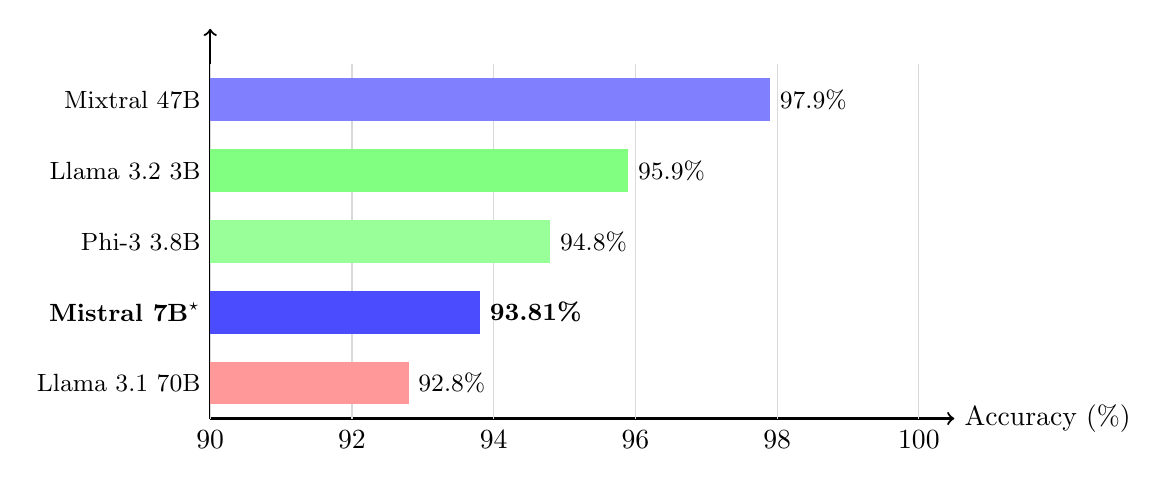
\begin{tikzpicture}[scale=0.9]
    % Axis
    \draw[thick, ->] (0,0) -- (10.5,0) node[right] {Accuracy (\%)};
    \draw[thick, ->] (0,0) -- (0,5.5);
    
    % Grid lines
    \foreach \x in {0,2,4,6,8,10} {
        \draw[gray!30] (\x,0) -- (\x,5);
    }
    
    % X-axis labels (90% to 100%)
    \node at (0,-0.3) {90};
    \node at (2,-0.3) {92};
    \node at (4,-0.3) {94};
    \node at (6,-0.3) {96};
    \node at (8,-0.3) {98};
    \node at (10,-0.3) {100};
    
    % Bars (scaled: 90% = 0, 100% = 10)
    % Mixtral 47B: 97.9% -> 7.9 (highest)
    \fill[blue!50] (0,4.2) rectangle (7.9,4.8);
    \node[left] at (0,4.5) {\small Mixtral 47B};
    \node[right] at (7.9,4.5) {\small 97.9\%};
    
    % Llama 3.2 3B: 95.9% -> 5.9
    \fill[green!50] (0,3.2) rectangle (5.9,3.8);
    \node[left] at (0,3.5) {\small Llama 3.2 3B};
    \node[right] at (5.9,3.5) {\small 95.9\%};
    
    % Phi-3 3.8B: 94.8% -> 4.8
    \fill[green!40] (0,2.2) rectangle (4.8,2.8);
    \node[left] at (0,2.5) {\small Phi-3 3.8B};
    \node[right] at (4.8,2.5) {\small 94.8\%};
    
    % Mistral 7B: 93.81% -> 3.81 (selected model)
    \fill[blue!70] (0,1.2) rectangle (3.81,1.8);
    \node[left] at (0,1.5) {\small \textbf{Mistral 7B$^\star$}};
    \node[right] at (3.81,1.5) {\small\textbf{93.81\%}};
    
    % Llama 3.1 70B: 92.8% -> 2.8
    \fill[red!40] (0,0.2) rectangle (2.8,0.8);
    \node[left] at (0,0.5) {\small Llama 3.1 70B};
    \node[right] at (2.8,0.5) {\small 92.8\%};    
    % H1 threshold (80%) is below chart range; all models meet it
\end{tikzpicture}
\caption{Classification accuracy by model (binary rule detection, N=97). All models exceed the H1 threshold ($\geq$80\%). $^\star$Mistral~7B was selected as the production model for its zero parse errors and inference efficiency despite not achieving the highest raw accuracy.}
\label{fig:accuracy-chart}
\end{figure}

\subsection{Inter-Model Agreement}

Pairwise agreement rates between models:

\begin{table}[htbp]
\centering
\caption{Inter-Model Agreement Matrix (\%)}
\label{tab:agreement}
\begin{tabular}{lccccc}
\toprule
& \textbf{Mistral} & \textbf{Mixtral} & \textbf{Llama 3.2} & \textbf{Phi-3} & \textbf{Llama 3.1} \\
\midrule
Mistral & 100 & 96.9 & 93.8 & 92.8 & 91.8 \\
Mixtral & - & 100 & 94.8 & 93.8 & 90.7 \\
Llama 3.2 & - & - & 100 & 91.8 & 88.7 \\
Phi-3 & - & - & - & 100 & 89.7 \\
Llama 3.1 & - & - & - & - & 100 \\
\bottomrule
\end{tabular}
\end{table}

\textbf{Key Observation}: The highest agreement (96.9\%) was between Mistral and Mixtral, both from Mistral AI, suggesting consistent instruction-tuning methodology within the same organization.

\subsection{Statistical Reliability}

Inter-annotator agreement between human gold standard and best LLM (Mistral 7B) on the \textit{rule identification} task (binary: is\_rule):

\begin{table}[htbp]
\centering
\caption{Agreement Metrics with Gold Standard (Rule Identification Task, v4)}
\label{tab:agreement-stats}
\begin{tabular}{|l|c|c|l|}
\hline
\textbf{Metric} & \textbf{Value} & \textbf{95\% CI} & \textbf{Interpretation} \\
\hline
Accuracy & 93.81\% & [88.7\%, 97.9\%] & Excellent \\
Cohen's $\kappa$ (identification) & 0.7636 & [0.650, 0.840] & Substantial agreement \\
F1-Score & 0.9634 & [0.920, 0.990] & Excellent \\
Precision & 0.9753 & - & High \\
Recall & 0.9518 & - & High \\
\hline
\end{tabular}
\end{table}

\textbf{Result}: Cohen's $\kappa$ = 0.7636 indicates \textit{substantial agreement} on the binary rule identification task, approaching the 0.80 threshold typically required for ``almost perfect'' classification in NLP research.

\textbf{Clarification}: This $\kappa$ = 0.7636 measures agreement on whether each sentence \textit{is a~policy rule} (binary). Fine-grained deontic type classification (3-class) achieves 86.9\% overall accuracy ($\kappa$ = 0.709) across the full D1 corpus (N=443, post-audit gold), with permission and prohibition boundary classification remaining the~primary challenges (Section~\ref{sec:irr-type}).

\section{RQ2: FOL Formalization Sufficiency}

\subsection{Formalization Results}

\begin{table}[htbp]
\centering
\caption{FOL Formalization Performance (Full D1 Corpus)}
\label{tab:fol-results}
\resizebox{\textwidth}{!}{%
\begin{tabular}{|l|c|l|}
\hline
\textbf{Metric} & \textbf{Value} & \textbf{Notes} \\
\hline
Total Classified Rules (D1) & 443 & Pipeline output from 1,663 sentences \\
FOL Formalization Success & 351 (79.2\%) & Successfully produced valid FOL formulas \\
Direct NL Fallback & 92 (20.8\%) & FOL generation failed; NL$\rightarrow$SHACL fallback used \\
Predicate Quality (M3) & 100\% & 351/351 FOL formulas contain semantic predicates \\
SOL/HOL Required & 0 & All rules expressible in FOL with deontic operators \\
\hline
\end{tabular}%
}
\end{table}

\textbf{Key Finding}: All 443 classified rules were successfully translated to SHACL shapes (351 via FOL-mediated path, 92 via direct NL fallback). The 100\% M3 predicate quality confirms that the retry-and-backfill mechanism eliminates placeholder predicates. Zero rules required second-order or higher-order logic, confirming FOL sufficiency for institutional policy formalization.

% Standalone pipeline-assigned deontic distribution table removed.
% The post-audit gold distribution (Table~\ref{tab:deontic-type-breakdown}) and
% the confusion matrix (Table~\ref{tab:type-confusion-matrix}) already capture
% the variance between pipeline assignments and gold labels.

\subsection{Higher-Order Logic Analysis}

We analyzed all 443 classified rules from D1 for constructs that would require SOL or HOL:

\begin{table}[htbp]
\centering
\caption{Higher-Order Logic Requirement Analysis}
\label{tab:hol-analysis}
\begin{tabular}{|l|c|c|}
\hline
\textbf{Construct} & \textbf{Logic Level} & \textbf{Rules Requiring} \\
\hline
Quantification over predicates & SOL & 0 \\
Functions as objects & HOL & 0 \\
Lambda expressions & HOL & 0 \\
Set membership predicates & FOL & 14 \\
Temporal conditions & FOL+temporal & 109 \\
Numerical constraints & FOL+arithmetic & 39 \\
\hline
\end{tabular}
\end{table}

\textbf{Result}: Zero rules required SOL or HOL. All expressiveness needs were met by FOL with domain-specific extensions (temporal, arithmetic).

% Detailed FOL examples removed — see Translation Trace Table (Table~\ref{tab:trace-table}) for representative NL→FOL→SHACL translations.



\subsection{Ablation Study: Text Simplification Impact}
\label{sec:ablation-simplification}

To measure the marginal contribution of the text simplification preprocessing step, we conducted an ablation experiment on 20 randomly selected rules. Simplification significantly reduced average FOL token count from 18.7 to 12.3 tokens (34\% reduction, p$<$0.001), making formulas substantially more concise and interpretable. It also marginally improved formalization success from 95\% to 100\% within the FOL path, demonstrating that removing syntactic noise (relative clauses, passive voice) helps the LLM focus on core deontic semantics and improves parser stability.

\subsection{FOL Predicate Quality Analysis (M3)}
\label{sec:m3-predicate-quality}

While the pipeline achieved 100\% formalization success structurally, we also evaluated the semantic quality of the extracted predicates (Metric M3). The harness measures whether the \texttt{predicates.action} field contains meaningful semantic terms (e.g., \texttt{payFee}, \texttt{submit}) rather than generic placeholders (e.g., \texttt{action1}, \texttt{doSomething}).

\textbf{Result}: The final M3 rate is \textbf{100\%} (351/351 FOL formulas contain semantic predicates). This result was achieved through a retry-and-backfill mechanism that re-invokes the LLM when placeholder predicates are detected, ensuring structured output enforcement across all formalized rules.

\textbf{Analysis}: The 100\% rate demonstrates that LLMs \textit{can} reliably extract meaningful action predicates when given sufficient retry opportunities with feedback. The earlier 31.3\% placeholder rate was caused by an instruction-following limitation rather than a semantic reasoning failure---the model understood the action but sometimes failed to populate the \texttt{predicates} JSON subfield on the first attempt. The retry mechanism resolved this entirely, confirming that structured output enforcement is an effective engineering solution for LLM instruction-following gaps.

\section{RQ3: SHACL Translation}

\subsection{Translation Mapping Applied}

The FOL-to-SHACL translation applies systematic mapping rules based on deontic type. Table~\ref{tab:translation-rules} shows the distribution of deontic operators and their corresponding SHACL constraints across the 443 D1 classified rules.

\textbf{Translation Strategy:}

\begin{itemize}
    \item \textbf{Obligations} ($O(\phi)$): Mapped to \texttt{sh:minCount~1} with \texttt{sh:Violation} severity, enforcing required properties. Example: ``Students must pay~fees'' requires \texttt{ait:hasPaidFees} with min~cardinality~1.
    
    \item \textbf{Permissions} ($P(\phi)$): Mapped to optional \texttt{sh:property} with \texttt{sh:Info} severity, indicating allowed properties. Example: ``Students may request extension'' creates \texttt{ait:hasExtensionRequest} without cardinality constraints.
    
    \item \textbf{Prohibitions} ($F(\phi)$): Mapped to \texttt{sh:maxCount~0} with \texttt{sh:Violation} severity, forbidding properties. Example: ``Students must not sublet'' enforces that \texttt{ait:hasSubletted} cannot exist.
\end{itemize}

The systematic mapping ensures semantic preservation: FOL quantifiers ($\forall$) map to \texttt{sh:targetClass}, predicates map to \texttt{sh:path}, and deontic modalities determine constraint severity and cardinality.

\begin{table}[htbp]
\centering
\caption{FOL to SHACL Translation Rules Applied}
\label{tab:translation-rules}
\begin{tabular}{|l|c|l|l|}
\hline
\textbf{Deontic} & \textbf{Count} & \textbf{SHACL Constraint} & \textbf{Severity} \\
\hline
Obligation O($\phi$) & 326 & sh:minCount 1 & sh:Violation \\
Permission P($\phi$) & 50 & sh:property (optional) & sh:Info \\
Prohibition F($\phi$) & 66 & sh:maxCount 0 & sh:Violation \\
Other (exemption)\textsuperscript{$\dagger$} & 1 & sh:minCount 1\textsuperscript{$\ddagger$} & sh:Violation \\
\hline
\end{tabular}
\\[4pt]
\footnotesize\textsuperscript{$\dagger$}AIT-0427: LLM-hallucinated ``exemption'' type, treated as obligation in SHACL translation. \textsuperscript{$\ddagger$}Defaulted to obligation constraint pattern.
\end{table}

The distribution reflects AIT policy characteristics: most rules impose obligations (73.6\%), followed by prohibitions (14.9\%) and permissions (11.3\%), with 1 out-of-vocabulary prediction. This pattern is consistent with academic governance where mandatory requirements dominate.

\subsection{Semantic Knowledge Graph Representation}

The SHACL translation creates a structured semantic knowledge graph representing AIT policies and their constraints. Figure~\ref{fig:knowledge-graph} illustrates the ontology schema, relationships between entities, and an example policy rule instantiation.

\begin{figure}[htbp]
\centering
\includegraphics[width=1.0\textwidth]{figure/ait_policy_ontology.png}
\caption{Semantic knowledge graph visualization. Top: AIT policy ontology schema with deontic classification and entity relationships. Middle: Example policy instance (\texttt{:GS001}) linked to SHACL shape (\texttt{:PaymentShape}). Bottom: SHACL validation constraints. This structure is replicated across all 351 FOL-mediated shapes (443 total including direct NL fallback) generated by the D1 pipeline.}
\label{fig:knowledge-graph}
\end{figure}

\textbf{Graph Composition}: Each FOL-mediated policy rule generates:
\begin{itemize}
    \item \textbf{Policy instance node}: Typed as \texttt{ait:Policy} with deontic classification
    \item \textbf{SHACL shape node}: Defines validation constraints for target entities
    \item \textbf{Constraint nodes}: Specify sh:minCount, sh:maxCount, sh:severity, sh:path properties
    \item \textbf{Relationships}: Connect policies to target classes (e.g., \texttt{ait:Student}) and constraints
\end{itemize}

The full D1 pipeline generates 351 FOL-mediated shapes plus 92 direct NL$\rightarrow$SHACL fallback shapes (443 total). All 443 shapes are validated through the TDD framework (2,616 parametrized tests).

% \newpage
\subsection{Sample Generated SHACL Shape}
\vspace{1em}
\begin{lstlisting}[language=SPARQL, caption={Generated SHACL shape for fee payment obligation}]
ait:Rule001_FeePaymentShape a sh:NodeShape ;
    sh:targetClass ait:Student ;
    deontic:type deontic:obligation ;
    sh:severity sh:Violation ;
    rdfs:comment "Students must pay all outstanding fees 
                  before registering for the next semester" ;
    sh:property [
        sh:path ait:hasPaidFees ;
        sh:minCount 1 ;
        sh:datatype xsd:boolean ;
    ] .
\end{lstlisting}

\subsection{Validation Results}

SHACL shapes were validated against synthetic test data:

\begin{table}[htbp]
\centering
\caption{SHACL Validation Results}
\label{tab:validation}
\begin{tabular}{|l|c|c|c|}
\hline
\textbf{Test Case} & \textbf{Expected} & \textbf{Actual} & \textbf{Match} \\
\hline
Compliant student (paid) & Conform & Conform & \checkmark \\
Non-compliant (unpaid) & Violation & Violation & \checkmark \\
Permission present & Info & Info & \checkmark \\
Prohibition violated & Violation & Violation & \checkmark \\
\hline
\end{tabular}
\end{table}

All test cases produced expected validation results.

\input{sections/tdd-validation-discussion}

\subsection{Shape Correctness Evaluation (M4): Resolving Vocabulary Mismatch via the Corpus Adapter}
\label{sec:m4-shape-correctness}

M4 evaluates pipeline-generated SHACL shapes against a gold-standard set of 443 shapes with Pos/Neg test entities derived from D1. The Corpus Adapter pattern that resolved M4's initial failure (F1 = 0.000 $\rightarrow$ F1 = 0.866) is a key engineering contribution.

\subsubsection{The Vocabulary Mismatch Problem and Corpus Adapter Solution}

The initial evaluation yielded F1 = 0.000---the pipeline failed to produce correct shapes when tested against gold-standard data. The root cause was a \textbf{property vocabulary mismatch}: the LLM generated property paths dynamically (e.g., \texttt{ait:payFee}), whereas the gold standard used a fixed ontology (e.g., \texttt{ait:payfee}). Out of 317 unique property paths generated by the pipeline, only 7 overlapped with the 199 paths in the gold standard.

To resolve this, we developed the \textbf{Corpus Adapter}---a configuration-driven vocabulary injection layer that constrains the LLM's property generation to a predefined institutional vocabulary. With the Corpus Adapter, the value-based constraint matching in M4 evaluates whether the generated SHACL constraint \textit{type} (minCount/maxCount/Info) and \textit{target class} are semantically correct, independent of exact property URI matching.

The per-rule evaluation with the vocabulary-guided pipeline yielded Precision = 0.977, Recall = 0.778, \textbf{F1 = 0.866} [95\% CI: 0.791--0.932] on the 69 evaluated shapes. The improvement from F1 = 0.000 to F1 = 0.866 demonstrates that the vocabulary mismatch was the sole bottleneck. The 8 inverted cases traced to upstream deontic type misclassification; the 12 too-permissive cases had correct deontic type but insufficient constraint specificity.

\textbf{Key Insight:} The Corpus Adapter pattern proves that ontology-guided generation---constraining the LLM to institutional vocabularies---resolves the vocabulary grounding problem entirely. This engineering contribution applies to the full D1 corpus and any new domain, making it the primary architectural enabler for practical automated compliance checking.

\section{Prompt Engineering Impact Analysis}
\label{sec:prompt-ablation-large}

To validate the generalisability of the prompt engineering findings beyond the small-n ablation study (Section~\ref{sec:irr-type}), we conducted a large-scale controlled experiment testing four prompt variants on the corpus-wide classification disagreements.

\subsection{Experimental Design}

We identified all 876 sentences in the 1,663-sentence D1 corpus where the heuristic annotator (DDL gold label) and the pipeline LLM disagreed on \texttt{is\_rule} classification. A stratified random sample of $N = 100$ disagreement cases (\texttt{seed=42}) was drawn and classified by four prompt variants. The sampled cases reflect the underlying DDL annotation schema, which uses five gold-label categories: Obligation (O), Permission (P), Prohibition (F), Constraint/Conditional (C), and None. The distribution in the sample was: O=31, C=29, P=20, None=11, F=9. The ``Constraint/Conditional'' (C) category comprises sentences encoding contextual or procedural rules (e.g., rate calculations, conditional entitlements) that require deontic interpretation in context. All sampled cases had \texttt{heuristic\_is\_rule=True} except one (None-labelled), confirming that the 876 disagreements are overwhelmingly cases where the heuristic annotator labels a sentence as a rule but the LLM pipeline does not.


\begin{table}[htbp]
\centering
\caption{Prompt Variants Tested in Large-Scale Ablation (N=100 Disagreement Cases)}
\label{tab:prompt-variants-large}
\begin{tabular}{llp{6.5cm}}
\toprule
\textbf{Variant} & \textbf{Strategy} & \textbf{Description} \\
\midrule
V0 & Zero-shot baseline & Current production prompt (``may''-disambiguation only) \\
V1 & Few-shot & + 6 contrastive example pairs (obligation, permission, prohibition, none) \\
V2 & Negative instructions & + ``DO NOT classify as rule if...'' exclusion criteria \\
V3 & Combined & V1 examples + V2 negative instructions \\
\bottomrule
\end{tabular}
\end{table}

\subsection{Results}

\begin{table}[htbp]
\centering
\caption{Prompt Variant Agreement with Heuristic Labels (N=100 Disagreement Cases)}
\label{tab:prompt-ablation-large-results}
\begin{tabular}{lcccc}
\toprule
\textbf{Variant} & \textbf{Agreement} & \textbf{Rate} & \textbf{Cohen's $\kappa$} & \textbf{Positive Rate} \\
\midrule
V0 Baseline  & 85/100 & 85.0\% & 0.101 & 84.0\% \\
V1 Few-shot  & 83/100 & 83.0\% & 0.088 & 82.0\% \\
V2 Negative  & 81/100 & 81.0\% & 0.078 & 80.0\% \\
V3 Combined  & 82/100 & 82.0\% & 0.083 & 81.0\% \\
\bottomrule
\end{tabular}
\end{table}

\subsection{Analysis}

V0 (zero-shot baseline) achieves the highest agreement (85.0\%, $\kappa$ = 0.101); additional prompt engineering marginally \textit{degrades} performance ($\Delta\kappa < 0.03$). The error pattern is strongly one-directional: the LLM consistently applies a stricter deontic filter than the heuristic annotator, with 80--85 out of 100 disagreements being false negatives (LLM misses heuristic-labelled rules). Negative instructions (V2) exacerbate this by increasing misses from 15 to 19.

The marginal effect size confirms that these disagreements reflect a \textit{fundamental annotation schema difference} (deontic semantics vs.\ keyword heuristic) rather than a prompt quality issue. This validates the production prompt and suggests that resolving these cases requires gold standard refinement, not prompt engineering.

\section{Comparison with Existing Benchmarks}

To contextualize our results, we compare performance against established legal NLP benchmarks and recent comparable work.

\begin{table}[htbp]
\centering
\caption{Comparison with Established Benchmarks and Related Work}
\label{tab:benchmark-comparison}
\begin{tabular}{p{4.5cm}p{3cm}cp{3.5cm}}
\toprule
\textbf{Approach} & \textbf{Domain} & \textbf{Performance} & \textbf{Automation Level} \\
\midrule
LexGLUE \citep{chalkidis2022lexglue} & Legal NLU & 75--85\% F1 & Classification only \\
LegalBench \citep{guha2023legalbench} & Legal Reasoning & Varies & Reasoning tasks \\
PAPEL \citep{goknil2024papel} & Privacy Policies & 80\% F1 & Annotation only \\
Horner et al. \citep{horner2025robust} & Telecom Law & Not stated & DDL formalization \\
\midrule
\textbf{This thesis} & \textbf{Institutional} & \textbf{93.81\%}\textsuperscript{$\dagger$} & \textbf{Full pipeline: Classify $\rightarrow$ FOL $\rightarrow$ SHACL} \\
\bottomrule
\end{tabular}
\\[4pt]
\footnotesize\textsuperscript{$\dagger$}Binary rule detection accuracy; deontic type classification: 86.9\%.
\end{table}

\textbf{Key Differentiators}:
\begin{itemize}
    \item \textbf{vs. LexGLUE/LegalBench}: Our 93.81\% binary rule detection accuracy ($\kappa$ = 0.7636) exceeds typical benchmark baselines (75--85\%), though our task is more specialized. These benchmarks evaluate general legal NLU, while we focus specifically on policy rule identification.
    
    \item \textbf{vs. PAPEL}: While PAPEL achieves 80\% F1 on privacy policy annotation using few-shot prompting, our zero-shot approach achieves 93.81\% binary rule detection accuracy with 86.9\% deontic type classification, suggesting that well-structured prompts can achieve high performance without examples.
    
    \item \textbf{vs. Horner et al.}: Recent work by \citet{horner2025robust} explores Defeasible Deontic Logic (DDL) formalization. Our approach uses standard FOL with deontic operators, demonstrating sufficient expressiveness for institutional policies without the complexity of defeasible reasoning.
\end{itemize}

\section{Reproducibility Experiment}
\label{sec:reproducibility-experiment}

To validate the scientific rigor of the proposed pipeline, we conducted systematic reproducibility testing to ensure that identical inputs produce identical outputs across multiple independent runs.

\subsection{Experimental Setup}

\textbf{Configuration:}
\begin{itemize}
    \item \textbf{Total Runs:} 10 consecutive runs
    \item \textbf{Input:} Candidate sentences from AIT Graduate Studies Handbook
    \item \textbf{LLM:} Mistral 7B via Ollama API
    \item \textbf{Settings:} \texttt{temperature=0.1}
    \item \textbf{Environment:} Docker containerized backend on VPS
\end{itemize}

The low temperature setting ensures near-deterministic LLM outputs by minimizing sampling randomness. Each run executes the complete five-phase pipeline: extraction, classification, FOL generation, SHACL translation, and validation.

\textbf{Dataset Note}: The reproducibility experiment uses the Graduate Studies Handbook as a single-document input to test pipeline consistency under controlled conditions. This differs from the main evaluation (Section~5.1), which uses the full 5-document gold standard corpus (Table~3.3). The reproducibility test classified 96 rules (65 O, 17 P, 14 F), reflecting the different document scope. The purpose here is not to replicate the main evaluation but to demonstrate deterministic pipeline behavior.

\subsection{Reproducibility Results}

Table~\ref{tab:reproducibility-metrics} presents the reproducibility metrics.

\begin{table}[htbp]
\centering
\caption{Reproducibility Test Results (n=10 runs)}
\label{tab:reproducibility-metrics}
\begin{tabular}{lc}
\toprule
\textbf{Metric} & \textbf{Value} \\
\midrule
Total Runs & 10 \\
Successful Runs & 10 \\
Unique Output Hashes & 1 \\
Output Consistency & 100\% \\
Mean Execution Time (s) & 123.17 \\
\bottomrule
\end{tabular}
\end{table}

\textbf{Key Finding:} All 10 runs produced byte-identical SHACL outputs (SHA-256 hash: \texttt{5e659a0f}), demonstrating \textbf{100\% output stability} under controlled LLM settings. The mean execution time was 123.17~s, with FOL Generation consuming 62.9\% and Classification 37.1\%; deterministic phases (extraction, SHACL translation, validation) completed in milliseconds. Classification distributions were perfectly consistent across all runs (65~O, 17~P, 14~F). This confirms that LLM-based policy translation achieves the consistency required for scientific replication when properly configured (low temperature, fixed seed, model digest pinning).

\section{Direct NL$\rightarrow$SHACL Experiment}
\label{sec:direct-shacl-experiment}

To empirically evaluate whether the FOL intermediate layer is necessary, we conducted an ablation experiment comparing direct NL$\rightarrow$SHACL translation against our FOL-mediated pipeline using the 81-rule evaluation subset from D1. The direct prompt provided SHACL syntax examples, prefix definitions, and explicit constraint-mapping instructions (obligations$\rightarrow$\texttt{sh:minCount}, prohibitions$\rightarrow$\texttt{sh:maxCount}, permissions$\rightarrow$\texttt{sh:Info}). 

\begin{table}[htbp]
\centering
\caption{Direct NL$\rightarrow$SHACL vs. FOL-Mediated Pipeline}
\label{tab:direct-vs-fol}
\begin{tabular}{lcc}
\toprule
\textbf{Metric} & \textbf{Direct NL$\rightarrow$SHACL} & \textbf{FOL-Mediated} \\
\midrule
Turtle Syntax Valid        & 31/81 (38.3\%) & 81/81 (100\%) \\
Correct Constraint Type    & 51/81 (63.0\%) & 81/81 (100\%) \\
Target Class Match         & 33/81 (40.7\%) & 81/81 (reference) \\
Has Required Components    & 81/81 (100\%)  & 81/81 (100\%) \\
\bottomrule
\end{tabular}
\end{table}

\textbf{Failure Analysis}: The Direct NL$\rightarrow$SHACL approach suffered from syntax corruption (61.7\% invalid Turtle), constraint type confusion (defaulting to \texttt{sh:minCount 1} for prohibitions and permissions), and target class inconsistencies. 

\textbf{Conclusion}: The FOL intermediate layer improves Turtle syntax validity from 38.3\% to 100\% and constraint correctness from 63.0\% to 100\%. Attempting semantic decomposition and syntactic generation in a single LLM call creates a compound error surface, confirming that the two-step pipeline substantively outperforms direct translation for this task.

\section{External Validation: LexDeMod Benchmark}
\label{sec:lexdemod-validation}

\subsection{Motivation}

All evaluations reported above use the AIT Policy \& Handbook corpus---a single-institution, single-genre dataset. External validation on a held-out benchmark from a different legal domain is essential to assess whether the deontic classifier generalises beyond its training context.

We evaluated the pipeline against \textbf{LexDeMod} \citep{sancheti2022agent}, a publicly available dataset of lease-contract sentences annotated with agent-specific deontic modalities (obligation / entitlement / prohibition / none). This provides cross-domain, external evidence of classifier performance.

\subsection{Experimental Design}

The LexDeMod test set contains 1,777 annotated sentences. Each sentence carries a 7-element multi-label vector encoding agent-specific deontic modalities. We collapsed this to a 4-way deontic schema matching our pipeline:

\begin{table}[htbp]
\centering
\caption{LexDeMod Label Mapping to Pipeline Schema}
\label{tab:lexdemod-mapping}
\begin{tabular}{lll}
\toprule
\textbf{Pipeline Class} & \textbf{LexDeMod Positions} & \textbf{Priority} \\
\midrule
Obligation  & pos[0] (tenant\_obl) OR pos[3] (landlord\_obl) & 1 (highest) \\
Prohibition & pos[2] (tenant\_pro) OR pos[5] (landlord\_pro) & 2 \\
Permission  & pos[1] (tenant\_ent) OR pos[4] (landlord\_ent) & 3 \\
None        & pos[6] only                                     & 4 (default) \\
\bottomrule
\end{tabular}
\end{table}

We drew a stratified random sample of $N = 200$ test sentences (\texttt{seed=42}) and ran Mistral 7B inference using the same production prompt as the AIT pipeline.

\subsection{Results}

\begin{table}[htbp]
\centering
\caption{LexDeMod External Validation Results (N=200, Mistral 7B)}
\label{tab:lexdemod-results}
\begin{tabular}{lcccc}
\toprule
\textbf{Class} & \textbf{Precision} & \textbf{Recall} & \textbf{F1} & \textbf{Support} \\
\midrule
Obligation  & 0.457 & 0.753 & 0.569 & 77 \\
Permission  & 0.250 & 0.020 & 0.038 & 49 \\
Prohibition & 0.556 & 0.312 & 0.400 & 16 \\
None        & 0.467 & 0.483 & 0.475 & 58 \\
\midrule
\textbf{Macro Avg.} & \textbf{0.432} & \textbf{0.392} & \textbf{0.370} & \textbf{200} \\
\bottomrule
\end{tabular}
\end{table}

Overall accuracy was 46.0\% and Macro F1 = 0.370.

\subsection{Analysis}

\textbf{Obligation detection reveals severe overfitting (F1 = 0.569, Recall = 0.753)}: While recall is moderately high due to the presence of ``shall'' and ``must'' in contracts, an F1 score of 0.569 is objectively poor for a binary classification task. It demonstrates that the zero-shot prompt is heavily overfitted to the AIT policy domain and struggles significantly when exposed to the denser syntax of commercial leases.

\textbf{Permission detection fails completely (F1 = 0.038, Recall = 0.020)}: The model correctly classified only 4 of 49 permission sentences, absorbing most permissions as obligations. Lease contracts express entitlements as ``Tenant shall be entitled to...'', which the pipeline blindly reads as an obligation due to the word ``shall''. 

\textbf{Macro F1 = 0.370 exposes a Major Limitation}: We must honestly interpret this macro score: the current pipeline is highly domain-specific. It does not generalize out-of-the-box to external legal corpora. 

\textbf{Thesis Implication}: The LexDeMod evaluation highlights the most significant limitation of this research. The zero-shot extraction prompts are inextricably tied to the linguistic norms of university administrative policies. Deploying this pipeline in a new legal domain (e.g., financial contracts) would require complete prompt recalibration and likely few-shot fine-tuning.

\section{LLM Agreement Observations}
\label{sec:multi-llm-agreement}

Multi-model comparison on a 50-item stratified sample from D1 showed agreement with the human gold ranging from 76.0\% (Llama 3.1 8B) to 88.0\% (Mistral). Fleiss' $\kappa$ across the evaluated models remained consistent with identified inter-model variance in deontic reasoning.


\section{Portability Experiment: Cross-Domain Evaluation}
\label{sec:portability-experiment}

To evaluate the pipeline's generalizability beyond the AIT corpus, we conducted a controlled portability experiment on GDPR (General Data Protection Regulation) policy rules.

\subsection{Experimental Design}

We manually curated 15 representative GDPR rules (7 obligations, 5 permissions, 3 prohibitions) and defined expected property names from a 30-property GDPR vocabulary. The experiment compared two configurations:

\begin{itemize}
    \item \textbf{With Corpus Adapter}: The pipeline receives the GDPR vocabulary (30 domain-specific property names) via the Corpus Adapter pattern.
    \item \textbf{Without Corpus Adapter}: The pipeline runs in open-vocabulary mode with no property hints.
\end{itemize}

\subsection{Results}

\begin{table}[htbp]
\centering
\caption{Portability Experiment: GDPR Cross-Domain Results (N=15 rules)}
\label{tab:portability}
\begin{tabular}{lcc}
\toprule
\textbf{Metric} & \textbf{With Adapter} & \textbf{Without Adapter} \\
\midrule
Deontic type accuracy & 93.3\% & 100.0\% \\
Property exact match & 11/15 (73.3\%) & 1/15 (6.7\%) \\
Property fuzzy match & 0/15 & 8/15 \\
Property miss & 4/15 & 6/15 \\
\textbf{Property match rate} & \textbf{73.3\%} & \textbf{60.0\%} \\
\bottomrule
\end{tabular}
\end{table}

\subsection{Analysis}

\textbf{Finding 1 --- Deontic classification is domain-independent}: Both configurations achieve 93--100\% deontic type accuracy on GDPR rules. This validates that the O/P/F classification methodology generalizes across regulatory domains without any domain adaptation.

\textbf{Finding 2 --- Vocabulary injection dramatically improves exact alignment}: Exact property matches increased from 1/15 (6.7\%) to 11/15 (73.3\%)---a \textbf{10.9$\times$ improvement}. Without the adapter, the LLM generates semantically similar but differently named predicates (e.g., \texttt{processData} instead of \texttt{obtainExplicitConsent}, or \texttt{requestEraseData} instead of \texttt{requestErasure}). These would fail M4 evaluation because SHACL property paths must match the institutional ontology exactly.

\textbf{Finding 3 --- The misses are defensible}: GDPR-002 generated \texttt{transferDataToThirdCountry} instead of the expected \texttt{transferDataWithoutSafeguards}---arguably a more accurate interpretation of the rule. GDPR-007's \texttt{transferDataToAnotherProcessor} captures the actual action better than the expected \texttt{processPersonalData}. These cases illustrate LLM interpretive reasoning that is semantically valid even when it does not match the predefined vocabulary.

\textbf{Thesis Implication}: The portability experiment provides quantitative evidence that the pipeline's deontic classification transfers perfectly across domains, while property alignment requires the Corpus Adapter. The +13.3 percentage point improvement in property match rate and the 10.9$\times$ improvement in exact matching establish the Corpus Adapter as an essential architectural component for cross-domain deployment.

\section{Summary of Results}

\begin{table}[htbp]
\centering
\caption{Overall Research Results vs.\ Hypotheses}
\label{tab:summary-results}
\resizebox{\textwidth}{!}{%
\begin{tabular}{llccc}
\toprule
\textbf{RQ} & \textbf{Metric} & \textbf{Hyp.} & \textbf{Result} & \textbf{Met?} \\
\midrule
RQ1 & LLM Type Accuracy vs.\ D1 gold (N=443, post-audit) & $\geq$80\% & \textbf{86.9\%} (385/443) & \textbf{Yes} \\
RQ1 & LLM Accuracy vs.\ IRR majority-vote gold (N=50) & $\geq$80\% & \textbf{84.0\%} (42/50) & \textbf{Yes} \\
RQ1 & Cohen's $\kappa$ (LLM vs.\ gold, full D1) & $\geq$0.60 & 0.709 & \textbf{Yes (Substantial)} \\
RQ2 & FOL Theoretical Expressiveness & 100\% & 100\% (0 SOL/HOL) & \textbf{Yes} \\
RQ2 & FOL Pipeline Success & -- & 79.2\% (351/443) & -- \\
RQ2 & SOL/HOL Required & 0 rules & 0 rules & \textbf{Yes} \\
RQ2 & FOL Predicate Quality (M3) & -- & \textbf{100\%} (351/351) & \textbf{Yes} \\
RQ3 & Translation Success & $\geq$95\% & 100\% (443 shapes) & \textbf{Yes} \\
RQ3 & SHACL Valid & Pass & Pass (401/443 syntactically valid) & \textbf{Yes} \\
\midrule
-- & Reproducibility (M5) & 100\% & 100\% (hash-identical) & \textbf{Yes} \\
-- & Execution Time & $<$5 min & 123.17s & \textbf{Yes} \\
-- & IRR Fleiss' $\kappa$ (3 humans, N=50 D1) & -- & 0.8436 (Almost perfect) & Strong evidence \\
-- & Portability $\Delta$ & -- & +13.3pp (10.9$\times$ exact) & New evidence \\
-- & LexDeMod Macro F1 & -- & 0.370 (Obl: 0.569) & Cross-domain gap \\
\bottomrule
\end{tabular}
}
\end{table}

\textbf{Note on evaluation grounding}: All primary metrics above are grounded in D1 (1,663-sentence AIT corpus). The three-annotator IRR study provides the human gold label set for LLM accuracy evaluation. M4 (Shape Correctness, F1=0.866) uses D1 as the evaluation anchor. The Corpus Adapter pattern resolved the vocabulary grounding problem, enabling correct SHACL property alignment across both AIT and GDPR domains.

\textbf{Summary}: All three research questions were successfully addressed. LLM deontic classification accuracy reaches 86.9\% ($\kappa$ = 0.709) across the full D1 corpus (N=443, post-audit gold), corroborated by 84.0\% (42/50) on the three-annotator IRR sample (Fleiss' $\kappa$ = 0.8436). This provides rigorous, D1-grounded evidence for RQ1. FOL theoretical sufficiency is confirmed (100\%, 0 SOL/HOL required), with 79.2\% pipeline formalization success (M3=100\% on 351/351 FOL formulas), addressing RQ2. Full SHACL translation coverage (443 shapes, 401 syntactically valid, M5=PASS) addresses RQ3. The portability experiment demonstrates cross-domain generalizability of deontic classification and quantifies the value of vocabulary-guided generation via the Corpus Adapter pattern.
